\documentclass[journal]{IEEEtran}
\usepackage{blindtext}
\usepackage{graphicx}
\usepackage{subfig}
\usepackage{caption}
\usepackage[english]{babel}
\usepackage{pinyin}
\usepackage{natbib}
\usepackage{notoccite}
\usepackage{amssymb}
\usepackage{textcomp}
\usepackage{floatrow}
\usepackage{amsmath}
%
\begin{document}
%
% paper title
\title{Real-Time Activity Classification by Match Filtering using Body-Worn Accelerometers}
%
\author{Craig~Euler, C.T.~Lin, Bryan~Juarez}
%
% make the title area
\maketitle
%
\begin{abstract}
Body worn sensors have been used in the market for many years now.
Many of which are used for activity monitoring or fitness.
In this paper, we make use of a matched-filtering algorithm for real-time activity classification from data obtained with three-axis accelerometers worn by the user.
We achieve invariance to sensor orientation with dimensionality reduction.
We make use of an instance-based learning algorithm to train the device to learn the individual's motion patterns and store that information as activity filters for our matched filter.
We improve computational efficiency with dimensionality reduction, temporal decomposition, and pre-processing of our filters for later use.
An assessment of our computational costs are provided as processing flop counts for the real-time specific parts of the algorithms.
\end{abstract}
%
\section{Introduction}
Various methods for activity classification using body-worn sensors exist.
Custom decision tree, automatically generated decision tree, and artificial neural networks \cite{parkka_ermes_korpipaa_mantyjarvi_peltola_korhonen_2006} have been explored as well as other frequency based classification methods \cite{sharma_purwar_lee_lee_chung_2008}.
In this paper, we make use of a matched-filter method to identify an individual\textquotesingle s activity in real-time.
The matched-filter method with use of thresholding and comparing the correlations of various filters is a simple method to use and have been studied in the past \cite{giannakis_tsatsanis_1990}.
Many of the algorithms and software structure were tailored to computational efficiency to accomidate the resource limitations on the MSP 432 micro-processor.
Having an a priori knowledge of the activity the individual is performing is useful for many current fitness algorithms.
Devices such as the Fit-Bit, Apple watch, Moov, Jawbone, etc. usually have the individual actively input the activity they are performing.

The algorithms described in this paper are broken into two main modules: Training the device to identify the user\textquotesingle s activity, and the real-time activity classification itself.

The training module does not need to be performed in real time.
This algorithm is the most demanding on computational resources and is only ran when training or re-training the unit to identify the user\textquotesingle s activity, so this can be performed on an external device such as a smart phone or tablet.
The purpose of the training module is to create the reference signal to be used on the micro-controller for real-time processing.

The second module is the real-time activity classification on the unit.
This module reads in the reference(s) stored on the unit to be used as templates that the matched-filter will use for determining the individual\textquotesingle s activity.
Both of these modules use the same principles and hence the same algorithm kernels.
%
\section{Algorithms}
\subsection{Activity Classification Method}
The matched-filter method is commonly used for extracting a signal out of noisy data.
We use this method for identifying a user\textquotesingle s activity from data generated by body-worn accelerometers.
Because the matched-filter method requires use of an existing reference template to identify the desired signal, we must develop our template from a training set.
We will discuss how we develop our set of templates for use in our matched-filter.

The matched filter is based on the cross correlation of the data $\textbf{y} = \{y\}_{k=0}^{N-1}$ with the reference signal $\textbf{x} = \{x\}_{k=0}^{M-1}$.
The cross correlation of $\textbf{x}$ with $\textbf{y}$ is defined as:
%
\begin{equation} \label{cross_correlation_eq}
(\textbf{x} \star \textbf{y}) = \left \{\sum_{i=0}^{M}x_{i} y_{i+k} \right \}_{k=0}^{N-M-1}
\end{equation}
%
which is simply a moving dot product.
We can then normalize \eqref{cross_correlation_eq} by the following:
%
\begin{equation} \label{norm_cross_correlation_eq}
\widehat{(\textbf{x} \star \textbf{y})}_k = \frac{(\textbf{x} \star \textbf{y})_k}{||\textbf{x}|| \ || \widetilde{\textbf{y}}_k || }, \quad k = 0,1,...,N-M-1
\end{equation}
%
where $|| \cdot ||$ is the usual $\ell_2$ norm and $\widetilde{\textbf{y}}_k = \{y_p\}_{p=k}^{M+k-1}$.
\eqref{norm_cross_correlation_eq} is now bounded by $[-1,1]$ and has any bias toward high energy removed.
We improve our computational efficiency by applying the convolution theorem to \eqref{cross_correlation_eq} and replacing it with:
%
\begin{equation} \label{conv_theorem}
(\textbf{x} \star \textbf{y}) = FFT^{-1}(FFT(\textbf{x}') FFT(\textbf{y})^*)
\end{equation}
%
Where $\textbf{x}'$ is $\textbf{x}$ that has been zero padded to the length of $\textbf{y}$ with the added restriction that the length of $\textbf{x}$ is no more than the length of $\textbf{y}$ and $FFT$ is the Fast Fourier Transform algorithm.
We are most interested where our reference $\textbf{x}$ best matches our data $\textbf{y}$.
We use the resulting max correlation to define our metric for  our matched-filter output as:
%
\begin{equation} \label{matched_filter_eq}
MF_{\textbf{x}}(\textbf{y}) := \underset{k \in [0, M-N)}{max} \left \{\widehat{(\textbf{x} \star \textbf{y})}_k \right \}
\end{equation}
%
If \eqref{matched_filter_eq} passes a threshold, the corresponding signal is a match.
%
\subsection{Dimensionality Reduction}
We manage to reduce our computational resources and remove our dependence on sensor orientation at the same time through a process of dimensionality reduction.
We assume that over a short period of time, a user\textquotesingle s limb movement is constrained mostly to a two-dimensional plane.
By identifying the plane of motion, we then project the acceleration data onto this plane and re-define our new axis accordingly.
By this assumption, activities that are mostly confined to two dimensions will improve our signal identification.

If we let $\textbf{a} = \{a_i\}_{i=0}^{N}$ represent our demeaned acceleration data over a specified time window in three dimensions then the covariance matrix of our acceleration data is represented by the real-symmetric $3 \times 3$ matrix $Q = \textbf{a} \textbf{a}^T$.
The resulting eigen vectors of this matrix are orthogonal and point in the directions where the data varies most [cite from some textbook here].
By projecting our data on the plain defined by the two most dominant eigen vectors, we effectively reduce our representation of our data to two dimensions.

To compute the matched-filter output for two dimensions, we generalize \eqref{matched_filter_eq} by augmenting our reference and data with both dimensions appropriately for normalization and adding together the cross correlations as:
%
\begin{equation} \label{cross_correlation_eq_2}
\widehat{(\textbf{x}^{1,2} \star \textbf{y}^{1,2})}_k^2 = \frac{(\textbf{x}^1 \star \textbf{y}^1)_k + (\textbf{x}^2 \star \textbf{y}^2)_k}{||[ \textbf{x}^1, \textbf{x}^2 ]|| \ || [ \widetilde{\textbf{y}}_k^1, \widetilde{\textbf{y}}_k^2 ] || },
\end{equation}
%
for $ k = 0,1,...,N-M-1 $.\\
%
\begin{equation} \label{matched_filter_eq_2}
MF_{\textbf{x}}^2(\textbf{y}) := \underset{k \in [0, M-N)}{max} \left \{\widehat{(\textbf{x} \star \textbf{y})}^2_k \right \}
\end{equation}
%
This works because both dimensions are always in phase with each other for any given activity which means that the match will happen in sinc.
%
\subsection{Decimation}
Decimation is the first step applied to our data before any additional processing takes place.
Decimation is a process of reducing the sampling rate of a signal.
The process consists of filtering to mitigate any possible aliasing distortion effects followed by a downsampling.
There is a tradeoff between performance and throughput when we decimate our signal, therefore, we use decimation solely for the purpose of improving our throughput.

For our application, we use a triangle filter prior to downsampling. This is achieved by convolving our data with the following weights:
%
\begin{equation} \label{trignal_filter_weights}
w_k^N =
\begin{cases}
  \frac{k+1}{N^2}, & \text{if}\ 0 \leq k < N \\
  \frac{2N - (k + 1)}{N^2}, & \text{if} N \leq k < 2N - 1
\end{cases}
\end{equation}
%
For a decimation value of $N$. Then the data is downsampled by $N$. This results in:
%
\begin{equation} \label{decimated_signal}
s_k^1 = \sum_{p=0}^{2N-1} w_{p+N(1-k)}^N s_{kN - (p+1)}^0 ?
\end{equation}
%
where $\{s_k^1\}_{k=0}^{M/N}$? is the decimated signal of $\{s_k^0\}_{k=0}^M$?.
\subsection{Training the Module}
We are able to identify an individual\textquotesingle s activity by matching the signal to a reference template.
For our application, we develop a reference signature for our matched filter directly from the person\textquotesingle s motion signature.
We do this by having the individual perform the specific activity over a specified amount of time and select the sub-interval of time that we find best represents the user's motion signature.
For a given activity, we attempt to find the representative periodic signal $s$ of our individual’s activity to be our template for our matched-filter.

If $\textbf{t} = \{t_k\}_{k=0}^{N_t}$ is our training set over $N_t$ data points, we define a collection of subsets $X$ of $\textbf{t}$:
%
\begin{equation} \label{X_subsets_of_training_eq}
X := \left \{ \{t_k\}_{k=p}^{p+M-1} | p=mI \right \}
\end{equation}
%
and $Y$ of $\textbf{t}$:
%
\begin{equation} \label{Y_subsets_of_training_eq}
Y := \left \{ \{t_k\}_{k=p}^{p+N-1} | p=nI \right \}
\end{equation}
%
where $M \leq N$, $I$ is a positive, fixed integer, and $(n,m) \in \mathbb{Z}^2$ where $(m,n)$ vary such that $0 \leq (m,n)I$ and $(m,n)I + (M,N) - 1 \leq N_t$. Then we can determine the representative signal $\textbf{s} \in X$ for our activity that satisfies the condition:
%
\begin{equation} \label{s_condition}
\sum_{y \in Y}MF^2_{\textbf{s}}(\textbf{y}) \geq \sum_{y \in Y}MF^2_{\textbf{x}}(\textbf{y}) \quad \forall \textbf{x} \in X
\end{equation}

We chose this method for its simplicity and robustness against outliers in our training set. We anticipate that the user will have idle motion at the start and end of their training duration when they activate the training mode and with possible disruptions during the process.
%
% Decimation with a tent filter for throughput performance
%
\section{Performance and Throughput}
%
The Kinetisense sensor was used for the performance analysis in this paper.
This unit has a three-axis accelerometer with an acceleration range of -5g to +5g and a sampling rate of 128Hz.
Samples of walking, jogging, and bicycling have been recorded with this unit for the purpose of analyzing the performance.
A separate instance of walking data has been used specifically for training the classifier.
In figure \ref{fig:MF_performance}, \subref{fig:frac_walking_jogging} and \subref{fig:frac_walking_bicycling} show the fraction of the correlation results that exceed the given correlation threshold when comparing the walking data reference to the given activity.
As we would expect, walking data matches better to walking data than the other activities.
ROC curves were produced from these corresponding results in \subref{fig:roc_walking_jogging} and \subref{fig:roc_walking_bicycling} to illistrate the effectiveness of the matched-filter as a classifier.
Figure \ref{fig:MF_performance} shows the comparison to bicycling.
Because the bicycling motions are considerably different from walking relative to jogging, we would expect better performance from bicycling.
%
%\begin{figure}[!tbp]
%\RawFloats
%  \centering
%     \begin{minipage}[b]{0.45\textwidth}
%        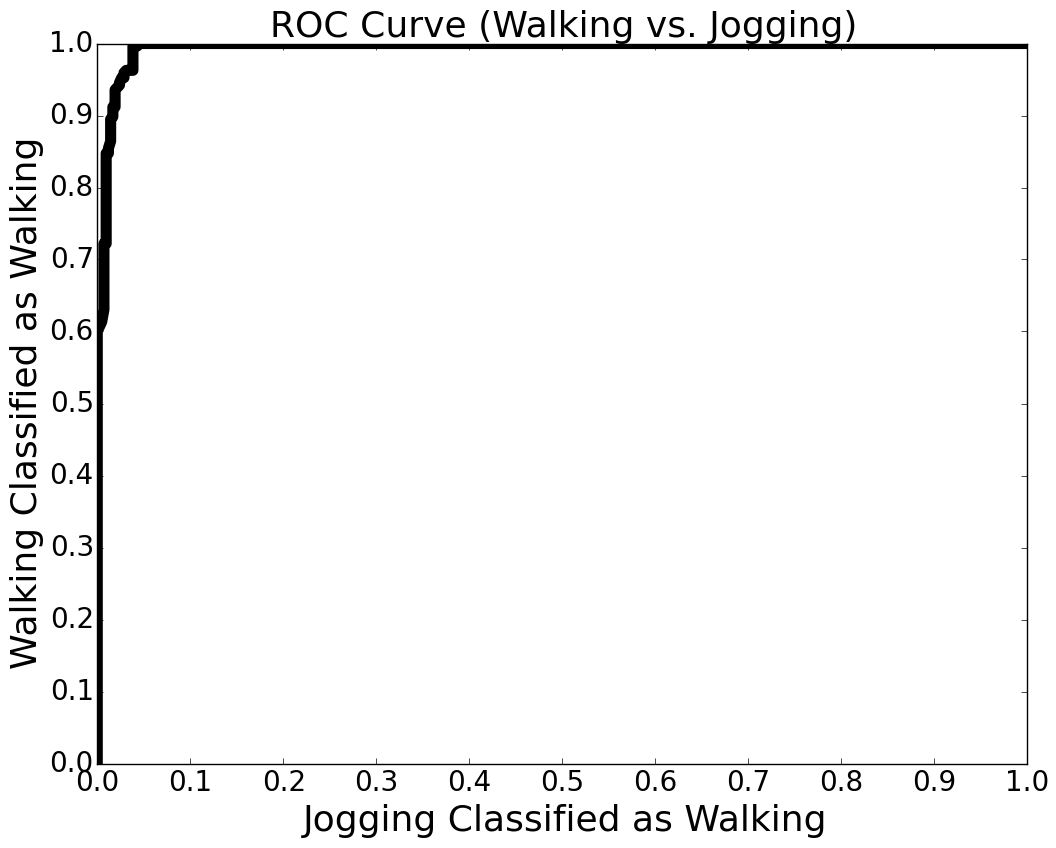
\includegraphics[angle=0,width=\textwidth]{ROC_walk_to_run.png}
%        \caption{\label{ROC_walk_to_run_fig}ROC curve with a downsample factor of 8}
%     \end{minipage}
%     \hfill
%     \begin{minipage}[b]{0.45\textwidth}
%     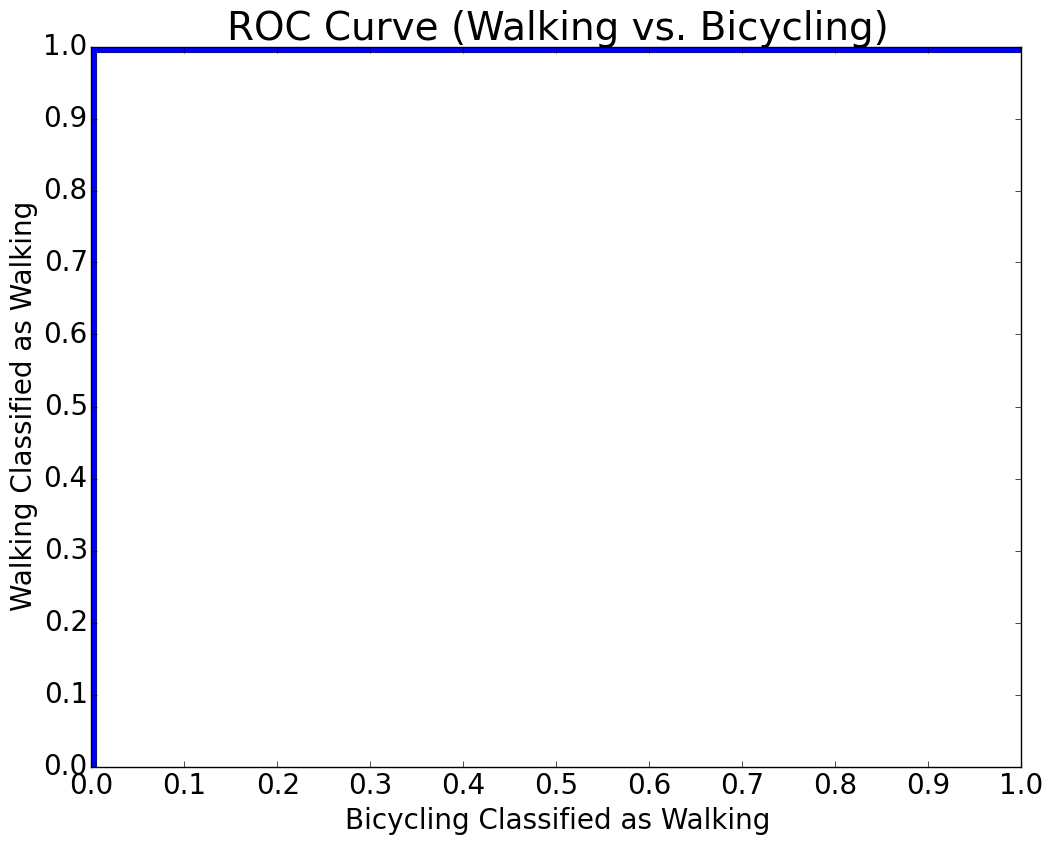
\includegraphics[angle=0,width=\textwidth]{ROC_walk_to_bike.png}
%        \caption{\label{ROC_walk_to_bike_fig}ROC curve with a downsample factor of 8}
%     \end{minipage}
%\caption{\label{ROC_walk_to_bike_fig}ROC curve with a downsample factor of 8}
%\end{figure}
%
\begin{figure}[!ht]
  %\captionsetup[subfigure]{labelformat=empty}
  \centering
  \subfloat[\label{fig:frac_walking_jogging}]{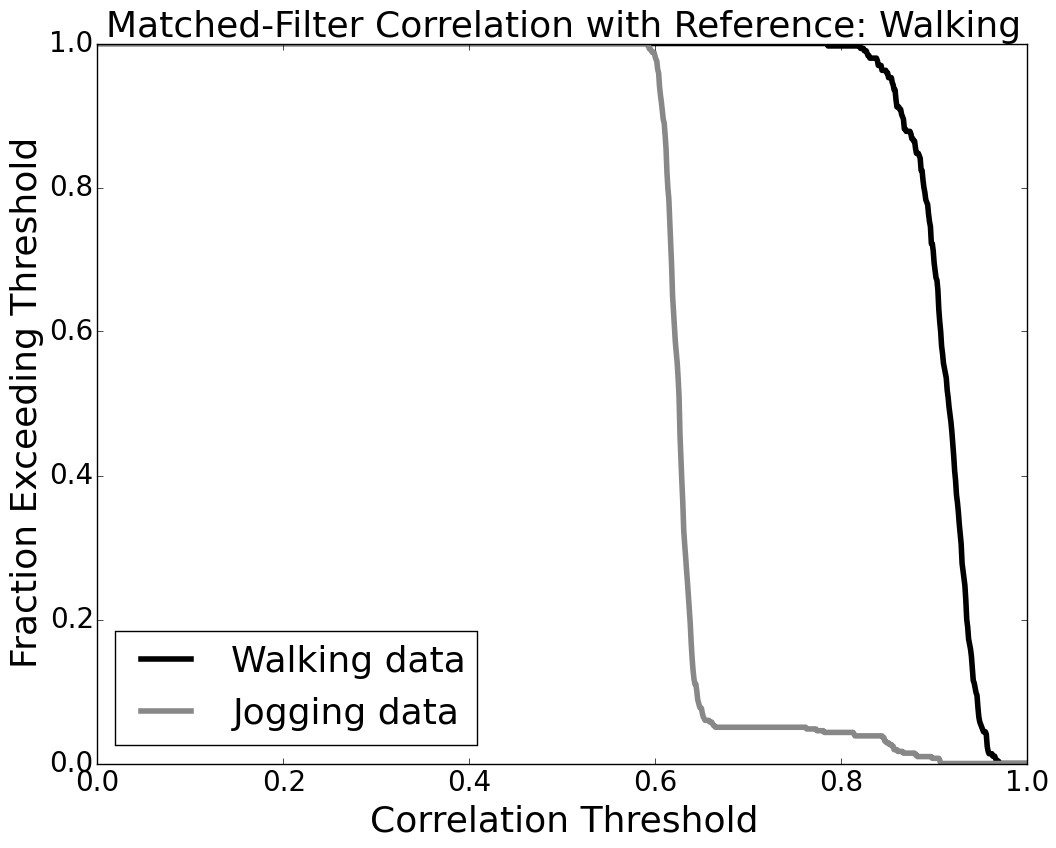
\includegraphics[width=.45\textwidth]{fraction_threshold_walking_to_jogging.png}}
  \quad
  \subfloat[\label{fig:frac_walking_bicycling}]{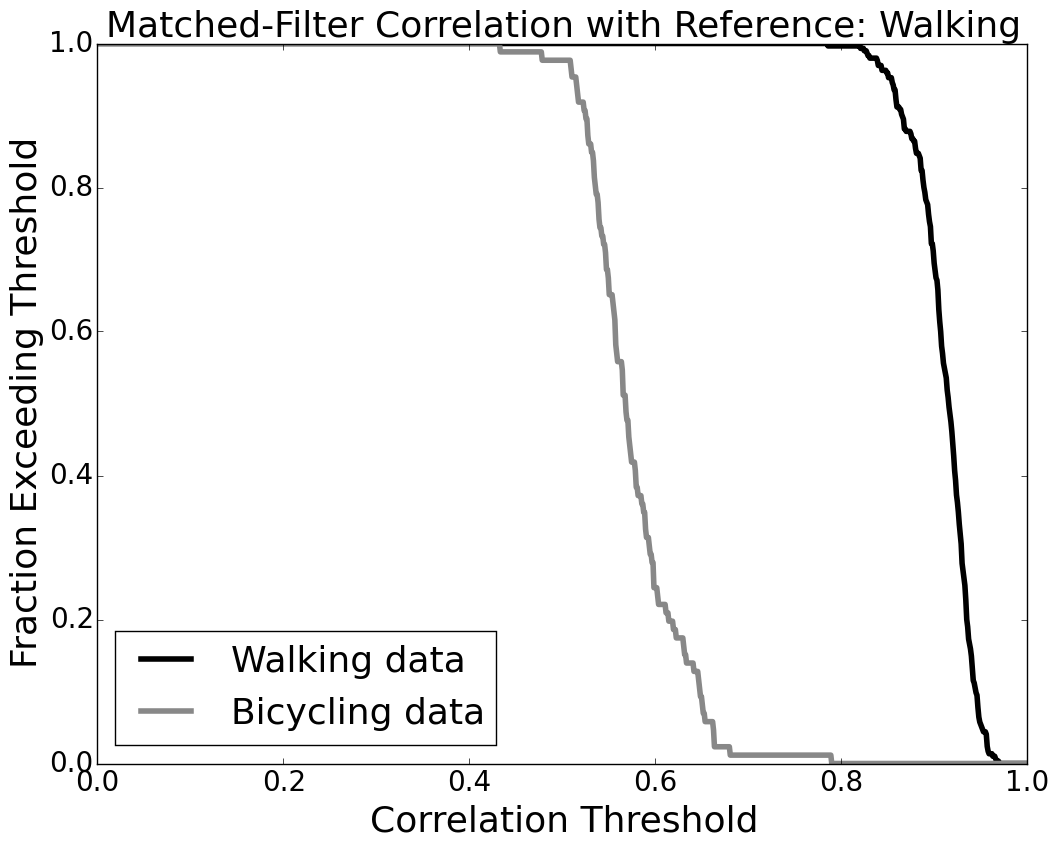
\includegraphics[width=.45\textwidth]{fraction_threshold_walking_to_bicycling.png}}
  \centering
  \quad
  \subfloat[\label{fig:roc_walking_jogging}]{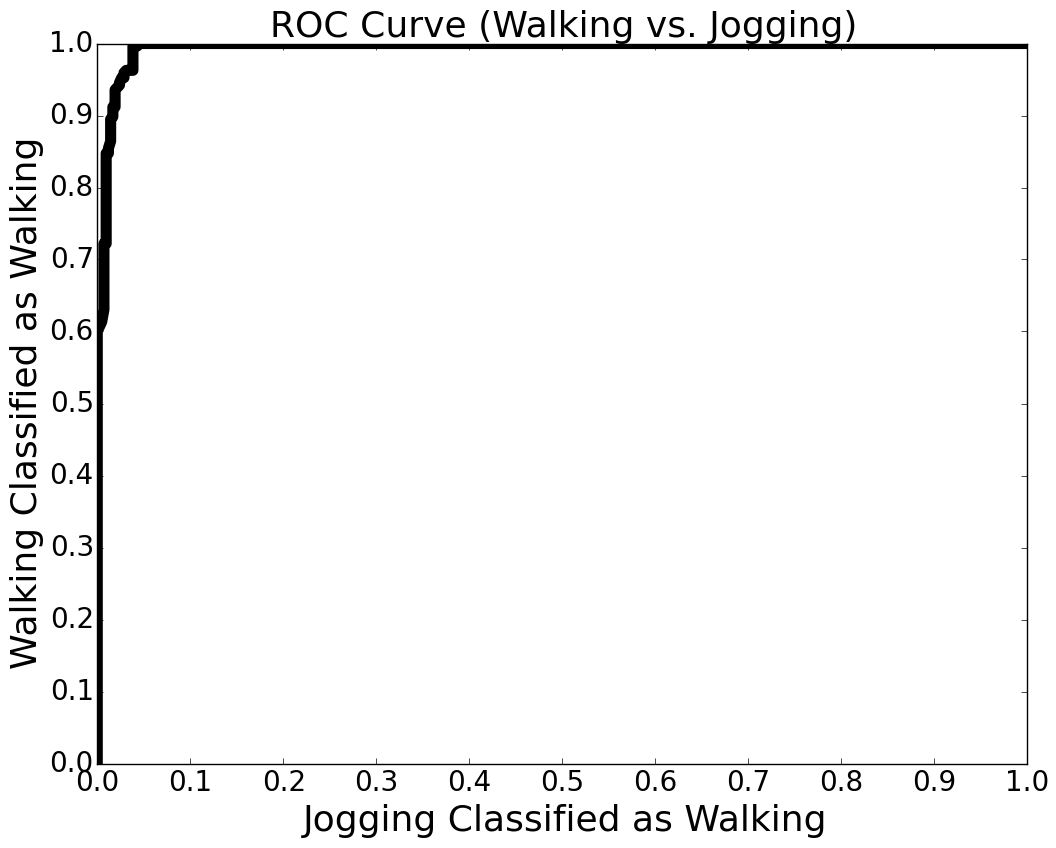
\includegraphics[width=.45\textwidth]{ROC_walk_to_run.png}}
  \centering
  \quad
  \subfloat[\label{fig:roc_walking_bicycling}]{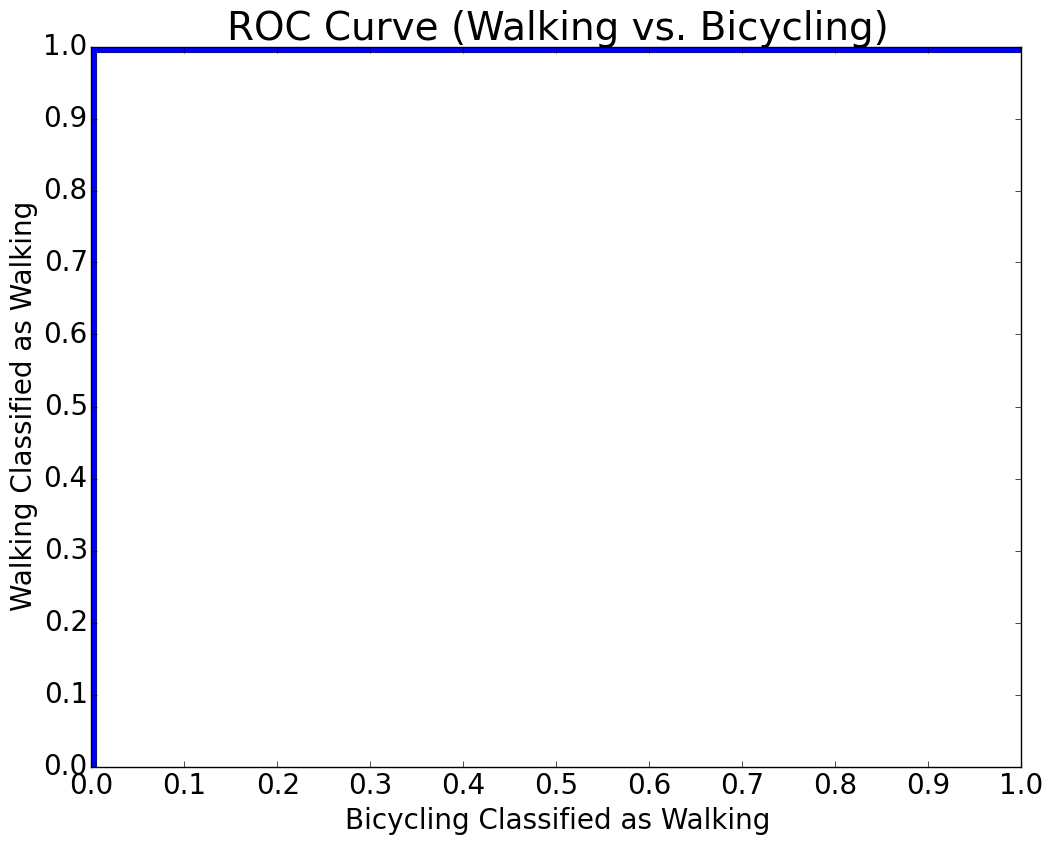
\includegraphics[width=.45\textwidth]{ROC_walk_to_bike.png}}
  \caption{Matched-filter performance comparing jogging and bicycling data against a reference for walking. Results produced with decimation 8}
  \label{fig:MF_performance}
\end{figure}
%
%\FloatBarrier
reference to figure \ref{fig:MF_performance}
%
\section{Conclusion}
conclusion text.
%
\appendices
%
\ifCLASSOPTIONcaptionsoff
  \newpage
\fi
%
\bibliographystyle{plain}
\bibliography{reference}
\end{document}
